{\bf BME154L - Spring 2012 - Exam \#2 Solutions}\hfill Name (Net ID):\underline{\hspace*{3.0in}}



\section{[15 points]}

\begin{center}
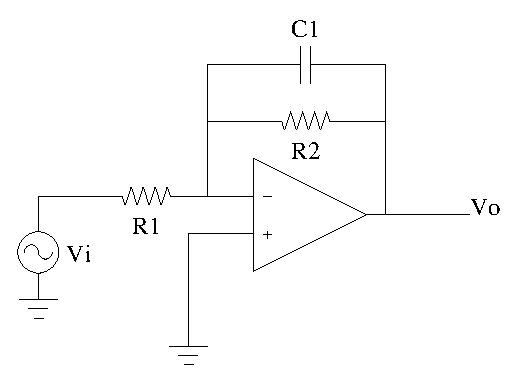
\includegraphics[width=0.4\linewidth]{active_lpf}
\end{center}

Given: $V_i(t)$ = 0.5 sin(200$\pi t$ + $\frac{\pi}{2}$) + 0.1 cos(2000000$\pi t$
+ $\pi$) V, $R_1$ = 10 k$\Omega$, $R_2$ = 20 k$\Omega$ and $C_1$ = 2 nF

\begin{enumerate}
    \item This circuit is a filter; what type/order filter is it?
    \item What is the filter's cutoff frequency(ies)?
    \item Sketch $V_o(t)$ for $t$ = [0:20] ms.
    \item Sketch $V_o(t)$ if the capacitor is removed from the circuit for $t$ = [0:20] ms.
\end{enumerate}

\clearpage

{\bf BME154L - Spring 2012 - Exam \#2 Solutions}\hfill Name (Net ID):\underline{\hspace*{3.0in}}



\clearpage
